\documentclass[pageno]{jpaper}

%replace XXX with the submission number you are given from the ISCA submission site.
\newcommand{\iscasubmissionnumber}{235}

\usepackage[normalem]{ulem}

\usepackage{graphicx}
\usepackage{fancybox}
\usepackage{pseudocode}
%\usepackage{subfigure}
\usepackage{cite}
\usepackage{xspace}

% Useful macros

\newcommand{\note}[1]{{\bf [ NOTE: #1 ]}}
\newcommand{\fixme}[1]{{\bf [ FIXME: #1 ]}}
\newcommand{\wunits}[2]{\mbox{#1\,#2}}
\newcommand{\um}{\mbox{$\mu$m}}
\newcommand{\xum}[1]{\wunits{#1}{\um}}
\newcommand{\by}[2]{\mbox{#1$\times$#2}}
\newcommand{\fix}[1]{\textcolor{red}{\bf #1}}
\def\eg{{\it e.g.}}

\newcommand{\todo}[1]{\noindent\textcolor{red}{[\underline{TODO}: #1]}}


% TODO: Use PACORA for the final version. SOSP uses double-blind review. 
%\newcommand{\tess}{Tessellation\xspace}
\newcommand{\pacora}{PACORA\xspace}


\begin{document}

\title{\pacora: Optimizing Resource Allocations for Dynamic Interactive Workloads}
\author{Authors Redacted}
\date{}
\maketitle

\thispagestyle{empty}

\begin{abstract}
\fix{rewrite duplicate sentences}

Modern computing systems are under intense pressure to provide guaranteed responsiveness to their workloads.  Ideally, applications with strict performance requirements should be given just enough resources to meet these requirements consistently, without unnecessarily siphoning resources from other applications. However, executing multiple parallel, real-time applications while satisfying QoS requirements is a complex optimization problem and traditionally operating systems have provided little support to provide QoS to applications.  As a result, client, cloud and embedded systems have all resorted to over-provisioning and isolating applications to guarantee responsiveness.  We present \pacora, a resource allocation framework, which is designed to provide responsiveness guarantees to a simultaneous mix of high-throughput parallel, interactive, and real-time applications in an efficient, scalable manner.  By measuring application behavior directly and using convex optimization techniques,  \pacora is able to understand the resource requirements of applications and performance near optimal resource allocation with low overhead. 

\end{abstract}


\section{Introduction}


The demands on modern systems have changed in the Post-PC era.  Users demand application responsiveness. These applications often deliver high-quality multimedia that require real-time guarantees.  Meeting this responsiveness goal is a challenge for all types of systems including cloud systems, databases, webservers, client operating systems, and emerging distributed embedded systems. Additionally, battery life and system power are extremely important, thereby forcing systems to try to find more efficient ways to meet the needs of their workloads.

Applications, jobs, or queries with strict performance requirements should ideally be given just enough system resources (\emph{e.g.} nodes, processor cores, cache slices, memory pages, various kinds of bandwidth) to meet these requirements consistently, without unnecessarily siphoning resources from other applications. However, executing multiple parallel, real-time applications while satisfying  \emph{Quality-of-Service} (QoS) requirements is a complex optimization problem, particularly as modern hardware diversifies to include a variety of parallel architectures (\emph{e.g.,} multicore, gpus).  Operating systems have historically not provided useful mechanisms that implement stronger performance guarantees and resource allocation has been rather unsystematic, making it difficult to reason about the expected response time of an application.

Consequently, responsiveness has been obtained at significant expense by designing for the worst case and over-provisioning.  Evidence of this behavior can be found in current systems of all sizes.  OSs attempt to describe responsiveness with a single value (usually called a \emph{priority}) associated with a thread of computation and adjusted within the operating system by a variety of \emph{ad-hoc} mechanisms. Other shared resources either employ independent machinery (\emph{e.g.} memory, caches), or are deemed so abundant as to require no explicit management at all (\emph{e.g.} I/O, network bandwidth).
 Priority approaches have no mechanism to describe deadlines or the resources required to meet them and so must run the highest priority applications as fast as possible on all the resources requested.   As a result, interactive and real-time applications are often run needlessly fast with significant over-provisioning --- wasting power and energy and preventing other applications from using the resources.

Some mobile systems have gone so far as to limit which applications can run in the background~\cite{iOsDev} in order to preserve responsiveness and battery life, despite the obvious concerns this raises for user experience.  Cloud computing providers routinely utilize their clusters at only 10\% to 50\% to keep the system responsive despite the additional operational costs of consuming electricity and the significant impact to the capital costs of the infrastructure~\cite{Barroso2009,Hennessy2011}.   In some cases, clusters only run a single application on each cluster to avoid unexpected interference.  Similarly the realtime community has used completely separate systems for each application to provide QoS despite the high cost of specialization and low utilization with this approach.

In this paper, we present \pacora, a resource allocation framework designed to provide responsiveness guarantees to a simultaneous mix of high-throughput parallel, interactive, and real-time applications in an efficient, scalable manner.  Unlike traditional systems, \pacora considers all resource types when making decisions and continuously determines the complete set of resources each application will use.   It maintains application-specific performance models through measurement to help determine resource requirements and responds to dynamic changes in both the deadlines and the relative importance of meeting each of them. It leverages convex optimization to determine the quantity of each resource to give each application. This lets the system make trade-offs among application QoS/responsiveness, system performance, and energy efficiency.

We believe \pacora is applicable to many resource allocation scenarios including cloud providers determining how much to give each job to avoid violating SLAs, databases allocating resources to queries, and distributed embedded systems allocating bandwidth among devices and sensors.  In this paper we choose to study client systems and their applications, implementing \pacora in a general-purpose operating system, because we believe this scenario has some of the most significant resource allocation challenges: a constantly changing environment requiring low overhead and fast response times, shared resources that create more interference among the applications, and platforms that are too diverse to allow \emph{a priori} performance prediction.
% applications that are more likely to be written by domain experts, thus less highly optimized.

\fix{Add Performance Numbers}

\section{\pacora Architecture}\label{sys_design}

%II.	System Architecture
%		i.	Application Specific
%		ii.	Resources Matter
%		iii.	Measurement
%		iv.	Optimization
%	a.	Convex by construction
%		i.	Fairly representative of the actual system
%			1.	(Systems should be more convex)
%		ii.	Low Overhead
%	b.	Explanation of resources
%	c.	Performance Models Built Online
%		i.	Explanation of performance
%		ii.	When does it run?
%	d.	Penalty functions
%	e.	Dynamic Optimization
%		i.	When does it run?


%\pacora, which stands for Performance-Aware Convex Optimization for Resource Allocation, is a framework designed to determine the proper amount of each resource type to assign to each application.  For our purposes an application is the entity to which the operating system allocates resources: it can viewed as a complete application (\emph{e.g.,} a video player) or a component of an application (\emph{e.g.,} a music synthesizer) or a process (\emph{e.g.,} indexing).

\pacora is a framework designed to determine the proper amount of each
resource type to give each application.  For example, consider a video
conference scenario where each participant requires a separate,
performance-guaranteed video stream.  New participants may join the
conference and others may leave, increasing or decreasing the number
of streams running at any given time.  Simultaneously, participants
may be collaborating through web browsers, or watching shared video
clips and web searching, while their systems run compute-intensive
background tasks such as updates, virus scans, or file indexing.
Although it may be relatively straightforward to provide
responsiveness guarantees for individual applications such as video
streams, the real challenge is to do so without reserving excessive
resources, which will compromise system utilization or power
consumption. The purpose of \pacora is to dynamically assign resources
across multiple applications to guarantee responsiveness without
over-provisioning and to adapt allocations as the application mix
changes.

For our purposes an application is an entity to which the system
allocates resources: these can be a complete application (\emph{e.g.,}
a video player), a component of an application (\emph{e.g.,} a music
synthesizer), a background OS process (\emph{e.g.,} indexing), a job
in warehouse-scale computing, or a distributed application in a
distributed embedded system.

\pacora is designed for systems where resource allocation is separated
from scheduling.  This split enables the use of application-specific
scheduling policies, which have the potential to be easier to design
and more efficient than general-purpose schedulers that have to work
for everything.  This approach leaves the system to focus on the
problem of \emph{how much} of each resource type to assign to each
application.  In client machines, \pacora is used to make coarse-grain
resource-allocation decisions (\emph{e.g.,} cores and memory pages) at
the OS level, while the micro-management of these resources to run
application tasks is left to user-level runtimes such as Intel
Threaded Building Blocks~\cite{CoMa08} or Lithe~\cite{lithe}, and to
user-level memory managers.
%As a result, \pacora could be used to consolidate realtime systems.  Resources can be allocated to various realtime user-level schedulers such as Earliest-Deadline-First or Rate-Monotonic schedulers, eliminating the need in the case of many applications for a realtime OS designed around one of these schedulers.
In the cloud environment, \pacora allocates
resources (\emph{e.g.,} nodes and storage) to jobs, and scheduling is
left to other entities such as the MapReduce framework\cite{mapreduce}
or the node OS.  \pacora can also be used in a hypervisor to allocate
resources among guest OSes.

\pacora formulates resource allocation as an optimization problem
built from two types of application-specific functions: a
response-time function and a penalty function. The response-time
function represents the performance of the application with different
resources, and is built with runtime measurements.  The penalty
function represents the user-level goals for the application
(\emph{i.e.,} the deadline and how important it is to meet). \pacora uses convex optimization\cite{BoVa} to
determine the ideal resource allocation across all active
applications.  The following subsections briefly introduce the primary
components of \pacora and the optimization formulation.

\subsection{Resources}

In our client system, resources are anything that the system can
``partition'' in hardware or software: specifically we use cores,
network bandwidth, cache ways, and memory pages in our system.
However, other resources could be easily added assuming they have QoS
enforcement mechanisms.  The other scenarios would have resources that
perform similar functions (compute, network, capacity), but at a
different scale. For warehouse-scale computing, resources are more
likely to be different types of nodes, network bandwidth, and
storage. For distributed embedded systems, resources would include
compute devices, link bandwidths, and memories.

\subsection{Response-Time Functions}

Response-time functions (RTF) represent the expected \emph{response
  time} of an application as a function of the resources allocated to
the application. The response time is an application-specific measure
of the performance of the application.  For example, the response time
of an application might be:
    \begin{itemize}\itemsep0pt \parskip0pt \parsep5pt
    \item The time from a mouse click to its result;
    \item The time to produce a frame;
    \item The time from a service request to its response;
    \item The time from job launch to job completion;
    \item The time to execute a specified amount of work.
    \end{itemize}

The RTFs are built to be convex functions.  All applications have a
function of the same form but the application-specific weights are set
using the performance history of the application.  RTFs are designed
to capture information such as how well an application scales with a
particular resource. As a result, RTFs naturally support
heterogeneity.  Each CPU or GPU type is simply viewed as a different
resource type by the system, and thus the RTFs will represent how
effectively an application uses a particular type of
core. Figure~\ref{sample_rtf} shows two example RTFs we have created
from applications we studied.

\begin{figure}[hb]
\includegraphics*[bb=0 0 360 360,width=.49\columnwidth]{bfs-fig.pdf}
\includegraphics*[bb=0 0 360
  360,width=.49\columnwidth]{streamcluster-fig.pdf}
\caption{\label{sample_rtf} Response Time Functions for a
  breadth-first search algorithm and streamcluster from PARSEC. We show two resource dimensions: cores and cache slices.}
\end{figure}

Equation~\ref{rtf_eq} below shows the RTF we use in \pacora.

\begin{equation}\label{rtf_eq}
\tau(w,a) = \tau_0 + \sum_{i\in n,j\in n}{\frac{w_{i,j}}{\sqrt{a_i * a_j}}}
\end{equation}

Here $\tau$ is the response time, $i$ and $j$ are
resource types, $n$ is the total number of resource types,
$a_{i}$ and $a_{j}$ are the allocations of resource types $i$
and $j$, and $w_{i,j}$ is the application-specific weight for
the term representing resources $i$ and $j$.
We choose this specific function because it is convex in the resources and in initial application studies
we found it models response time behavior accurately enough to allow the optimization to make good decisions.
In our experience the cross term weights (those with $i\neq j$) are almost always negligible and can be omitted.
The dimensionality of the function increases roughly linearly with the number of resource types.
The RTFs will be described further in Section~\ref{RTFs}.
Alternative models and the initial model evaluations are described in
\cite{pacora_tr}.
%Appendix~\ref{rtf_choice}.


\pacora assumes some amount of performance isolation between
applications.  In order for the RTFs to accurately reflect the
expected response times of the applications, it is important that the
response time does not change much as a function of the other
applications currently running on the machine.  However, the
performance isolation need not be completely perfect: all of our
evaluation was run on current x86 hardware with some shared resources,
and \pacora is still effective. Section~\ref{discuss} discusses
handling shared resources in more detail.

\subsection{Penalty Functions}
Penalty functions are designed to represent the user-level goals of
the application. They are similar to priorities but are functions of
the response time rather than simply values, so they can explicitly
represent deadlines.  Knowing the deadlines lets the system make
optimizations that are difficult in today's systems, such as running
just fast enough to make the deadline. Like priorities, the penalty
functions are set by the system on behalf of the user.

\pacora's penalty functions $\pi$ are non-decreasing piecewise-linear
functions of the response time $\tau$ of the form $\pi(\tau) = \max(0, (\tau - d)s)$
where $d$ represents the deadline of the application and $s$ (slope)
defines the rate the penalty increases as response time increases. For
applications without response-time constraints the deadline can be set
to $0$. Two representative graphs of this type appear in
Figures~\ref{f:pen1} and~\ref{f:pen2}.

%In a client operating system, management of penalty function modifications
%should be highly automated by the system to avoid unduly burdening the user.
%As an application grows or diminishes in importance, its penalty function can be modified accordingly.
%Adjustment is also likely to occur in transitions between operating scenarios.
%For example, when unplugging a device all of the background activities could have their slopes significantly reduced to save battery life.

\begin{figure}[hb]
\parbox{1.6in}{
\includegraphics*{Penalty1.eps}
\caption{\label{f:pen1}A penalty function with a response time constraint.}
}
\hspace{\fill}
\parbox{1.6in}{
\includegraphics*{Penalty2.eps}
\caption{\label{f:pen2}A penalty function with no response time constraint.}
}
\end{figure}

\subsection{Resource Allocation as Optimization}

\pacora formulates resource allocation as an optimization problem
designed to minimize the total penalty of the system. This approach is
analogous to minimizing user dissatisfaction with the user experience
due to missed deadlines in a client system, and minimizing the contract
penalties paid for violated SLAs in a cloud
system.

The optimization selects the allocations for all resources and
resource types at once.  This approach enables the system to make
tradeoffs between resource types.  For example, the system could
choose to allocate more memory bandwidth in lieu of on-chip cache, or
one large core instead of several small cores.  Given that all of the
resources allocated to an application contribute to the response time,
it would difficult to provide predictable response times for
applications by considering the allocation of only one resource type at a
time.

A succinct mathematical characterization of this resource allocation scheme is the following:
\begin{eqnarray*}
& \makebox[1in][r]{Minimize}   & \sum_{p\in P} {\pi_p(\tau_p(a_{p,1}\ldots a_{p,n}))}  \\
& \makebox[1in][r]{Subject to} & \sum_{p\in P} a_{p,r} \leq A_r, r = 1,\ldots n        \\
& \makebox[1in][r]{and}        & a_{p,r} \geq 0
\end{eqnarray*}
Here $\pi_p$ is the penalty function for application $p$,
$\tau_p$ is its response time function,
$a_{p,r}$ is the allocation of resource $r$ to application $p$,
and $A_r$ is the total amount of resource $r$ available.  Optimization details are described in Section~\ref{dyn_opt}.

\subsection{Convex Optimization}

If the penalty functions, response time functions, and resource
constraints were arbitrary, little could be done to optimize the total
penalty beyond searching at random for the best allocation.  However,
by framing our resource allocation problem as a \emph{convex
  optimization problem}\cite{BoVa}, two benefits accrue: an optimal
solution will exist without multiple local extrema, and fast,
incremental solutions will become feasible.

A constrained optimization problem is \emph{convex} if both the objective function to be minimized
and the constraint functions that define its feasible solutions are convex functions.
A function $f$ is convex if its domain is a convex set and
$f(\theta x + (1-\theta)y) \leq \theta f(x) + (1-\theta)f(y)$
for all $\theta$ between 0 and 1.
A set is convex if for any two points $x$ and $y$ in the set, the point
$\theta x + (1-\theta)y$
is also in the set for all $\theta$ between 0 and 1.
%If $f$ is differentiable, it is convex if its domain is an open convex set and
%$f(y) \geq f(x) + \nabla f^T\cdot(y-x)$ where $\nabla f$ is the gradient of $f$.
%Put another way, $f$ is convex if its first-order Taylor approximations
%are always global underestimates of its true value.

A convex optimization problem is one that can be expressed in this form:
\begin{eqnarray*}
& \makebox[1in][r]{Minimize}   & f_0(x_1,\ldots x_m)                              \\
& \makebox[1in][r]{Subject to} & f_i(x_1,\ldots f_m) \leq 0, i = 1,\ldots k        \\
& \makebox[1in][r]{where}      & \forall i \quad f_i:\Re^m \rightarrow \Re \mbox{ is convex.}
\end{eqnarray*}


\pacora's resource allocation problem can be transformed into a convex
optimization problem in the $m = |P|\cdot n$ variables $a_{p,r}$ as
long as the penalty functions $\pi_p$ are convex non-decreasing and
the response-time functions $\tau_p$ are convex.  We designed our
functions to meet these constraints, and proofs of their convexity can
be found in~\cite{pacora_tr}.
%Appendix~\ref{convex}. 
Note that the resource constraints
are affine and therefore convex; they can be rewritten as $\sum_{p\in
  P} (a_{p,r} - A_r) \leq 0$ and $-a_{p,r} \leq 0$.

The convex formulation makes the optimization scale linearly in the
number of resource types and the number of applications.  For client
operating systems with around 100 applications running and 10 resource
dimensions, the total number of variables in the optimization problem
is 1000---a very small problem which is solved in microseconds on
current systems.  Cloud systems could have many more than 100
applications running, but the problem size scales linearly and the
potential benefits of a good allocation should scale rapidly with the
size of the system.

\pacora also formulates RTF \emph{creation} as a convex optimization
problem, as explained in Section~\ref{RTFs}.

\subsection{Power and Energy}
In \pacora, we create an artificial application to represent the
interest in reducing system power and energy.  Application 0 is
designated the idle application and receives allocations of all
resources that are left idle, \emph{i.e.,} not allocated to other
applications.  The idle resources can be powered off or put to sleep
if possible to save power.

The ``response time'' for application 0, $\tau_0$, is artificially
defined to be the total system power consumption.
%This response function is affine and monotone nonincreasing in its arguments $a_{0,r}$.
The penalty function $\pi_0$ establishes a system tradeoff between
power and performance that will determine which resources are
allocated to applications to improve performance and which are left
idle.  The penalty function $\pi_0$ can be used to keep total system
power below the parameter $d_0$ to the extent the penalties of other
applications cannot overcome its penalty slope $s_0$. Both $s_0$ and
$d_0$ can be adjusted to reflect the current battery charge in mobile
devices. For example, as the battery depletes, $d_0$ could be decreased or $s_0$ increased
to force other applications to slow or cease execution.

%Additionally, application 0 functions as \emph{slack} variables in our optimization problem turning the resource bounds into equalities:
%\begin{equation}
%\sum_{p\in P} a_{p,r} - A_r = 0, r = 1,\dots n.
%\end{equation}




\section{Response Time Functions}\label{RTFs}
%III.	Application Functions
%	a.	Resource Value Functions
%		i.	Structure
%		ii.	Model Building Approach
%			1.	Who measures the data?
%	b.	Penalty Functions
%		i.	Where do the deadlines come from?
%		ii.	How do we set the slopes?
%	c.	Power Model


In this section, we describe the design of \pacora's RTFs in more detail.
RTFs describe an application's performance given its resource assignments.  These functions capture information about the performance impact of a particular resource to an application on the current hardware at a particular time. Without this information, it would be difficult for any resource allocation system to make informed decisions short of blindly trying a variety of allocations and picking the best one.

\subsubsection*{Modeling versus Interpolating} While it might have been possible to model response times by recording past values and interpolating among them, this idea has serious shortcomings:
\begin{itemize}
\item The multidimensional response time tables would be large;
\item Interpolation in many dimensions is computationally expensive;
\item The measurements will be noisy and require smoothing;
\item Convexity in the resources may be violated;
\item Gradient estimation will be slow and difficult.
\end{itemize}

Instead of interpolating, \pacora maintains a parameterized analytic response time model with the partial derivatives evaluated from the model \emph{a priori}. Application responsiveness is highly nonlinear for an increasing variety of applications like streaming media or gaming, thus requiring many data points to represent the response times without a model. Using models, each application can be described in a small number of parameters.  Models can be built from just a few data points and can naturally smooth out noisy data. Their gradients, needed by \pacora to solve the optimization problem efficiently, are easy to calculate.

\pacora models response times with functions that are convex by construction.
The specific function chosen for \pacora is shown in Equation~\ref{rtf_eq} above.
In this equation, the response time is modeled as a weighted sum of component terms,
roughly one per resource, where a term $w_i/a_i$ is the amount of work $w_i \geq 0$
divided by $a_i$, the allocation of the $i$th resource~\cite{Snav}.
For example, one term might model instructions executed divided by total processor MIPS;
another might model network accesses divided by bandwidth, and so forth.
%Asynchrony and latency tolerance may make response time components overlap partly or fully; and thus we added additional terms to represent the interactions between resources.

Such models are automatically convex in the allocations because $1/a$ is convex for positive $a$ and because a positively-weighted sum of convex functions is convex.  The models are also linear in the weights.

%It is obviously important to guarantee the positivity of the resource allocations. This guarantee can be enforced as the %allocations are selected during penalty optimization, or the response time model can be made to return $\infty$ if any allocation %is less than or equal to zero. This latter idea preserves the convexity of the model and extends its domain to all of $\Re^n$ and %consequently we used this approach in our implementation.
%The gradient $\nabla\tau$ is needed by the penalty optimization algorithm.
%Since $\tau$ is analytic, generic, and symbolically differentiable
%it is a simple matter to compute the gradient of $\tau$ once the model is defined.

\subsubsection*{Non-Convexity}
Forcing RTFs to be convex assumes that the actual response times are close to convex. We find this to be a plausible requirement as applications almost completely follow the proverbial ``Law of Diminishing Returns'' for resource allocations.

However, there are examples of response time versus resource behavior that violate convexity.   For example, we have seen non-convex performance in applications when dealing with hyperthreads or memory pages.  For two of our applications, 5 hyperthreads resulted in significantly worse performance than either 4 or 6.  When studying some other applications, we found that particular numbers of memory pages, (\emph{e.g.,} 2K), resulted in much better performance than the adjacent page allocations.  Outliers and additional challenges to response time modeling are discussed in Section~\ref{discuss}.
%Avoiding (or seeking out) these allocations would add significant cost to the optimization problem.

Another kind of convexity violation can occur in memory allocation, where ``plateaus'' can sometimes occur as in Figure~\ref{f:plat}. Such plateaus are typically caused by adaptations within the application (\emph{e.g.,} adjusting the algorithm or output quality).
%to accommodate variable resource availability.  
The response time is really the \emph{minimum} of several convex functions depending on allocation, and the point-wise minimum that the application implements fails to preserve convexity.  The effect of the plateaus will be a non-convex penalty as shown in Figure~\ref{f:plateffect} and multiple extrema in the optimization problem will be a likely result. 



\begin{figure}[hb]
\parbox{1.6in}{
\includegraphics*{Plateau1.eps}
\caption{\label{f:plat}Response time function with some resource ``plateaus''.}
}
\hspace{\fill}
\parbox{1.6in}{
\includegraphics*{Plateau2.eps}
\caption{\label{f:plateffect}Net effect of the resource plateaus on the application penalty.}
}
\end{figure}
There are several ways to avoid this problem.  One is based on the observation that such response time functions will at least be \emph{quasiconvex}.  Another idea is to use additional constraints to explore convex sub-domains of $\tau$. Either approach adds significant computational cost, and we found that our simple convex models still resulted in high-quality resource allocations. Thus we chose not to implement any of these approaches.  Alternative approaches to handling non-convex behavior are described in~\cite{pacora_tr}. 

%\subsubsection*{Dynamically Changing Applications}
%
%
%\fix{changing apps}
%\fix{dynamic compilation}
%\fix{phases}
%Response time will commonly vary with time as a application changes phase and makes better or worse use of its resources.
%\fix{non-determinism}
%
%\fix{Input Variability}


\subsubsection*{Data Collection and Model Creation Time}
There are many ways to collect the response time data for applications. The user-level runtime scheduler is one possible source, or the operating system could measure progress using performance counters.  In our implementation, applications report their own measured values; however, this solution was chosen simply as a way to test the validity of the concept.  In a production operating system it may not be a good idea because applications could lie about their performance.  In a datacenter environment this might be less of a concern.

There are also many different possible moments to create response time functions.  RTFs could be created in advance and distributed with the application. This approach could make lots of sense for app stores since most of them cater to just a few platforms. RTFs could also be crowd-sourced and built in the cloud, which has the advantage making it easy to collect a diverse set of training points.  However, all of these approaches lack adaptability.  As a result, we have chosen to implement two solutions that collect data directly from the user's machine.  The first approach is to adapt to the system by collecting all of the training points at application install time and building the model then.  The most highly adaptive approach collects data continuously as the application runs, uses the data to modify the model training set, and rebuilds the model.  A hybrid approach may be the most effective: applications can begin with a generic model and improve it over time. The remainder of this Section describes our model creation process in detail.
\subsection{Response Time Model Creation}
To create RTF models either at install time or online we use a convex least squares approach described below.  For the install time approach we use a genetic algorithm, Audze-Eglasis Design of Experiments\cite{bates-aes03}, to select the resource vectors to use for training.  These vectors and their response times are fed into the convex least squares algorithm. In the online approach the data comes from the application's response time history.

\subsubsection*{Least Squares Minimization}
After enough measurements, discovery of the model parameters $w$ that define the function $\tau$
can be based on a solution to the over-determined linear system $t=Dw$,
where $t$ is a column vector of actual response times measured for the application
and $D$ is a matrix whose $i$th row $D_{i,*}$ contains the corresponding resource vector.
Estimating $w$ is relatively straightforward: a least-squares solution accomplished via
\emph{QR factorization}\cite{GoVL} of $D$ will determine the $w$ that minimizes the \emph residual error of
$\|Dw - t\|^2_2 =  \|Rw - Q^Tt\|^2_2$.
%The solution proceeds as follows:
%\begin{eqnarray*}
%t     &=& Dw  - \varepsilon    \\
%      &=& QRw - \varepsilon    \\
%Q^Tt  &=& Rw  - Q^T\varepsilon
%\end{eqnarray*}
%
The individual elementary orthogonal transformations, \emph{e.g.,} Givens rotations,
that triangularize $R$ by progressively zeroing out $D$'s sub-diagonal elements are simultaneously applied to $t$.
%The elements of the resulting vector $Q^Tt$ that correspond to zero rows in $R$ comprise $-Q^T\varepsilon$.
%Since $Rw$ exactly equals the upper part of $Q^Tt$, the upper part of $Q^T\varepsilon$ is zero. The residual error for the %$t_i$
%can be found by premultiplying $Q^T\varepsilon$ by $Q$.

%This formulation assumes a model norm $p = 1$. If a different model norm $p$ is desired, such as $p = 2$, we could first square %each measurement in $t$
%and each reciprocal bandwidth term in $D$ and then follow the foregoing procedure.
%The elements of the result $w$ will be squares as well, and the 2-norm of the difference in the squared quantities will be %minimized.  This is not the same as minimizing the 4-norm; what is being minimized is $1/2\|\mbox{diag}(Dww^TD^T - tt^T)\|^2_2$.

\subsection{On-line Response Time Modeling}
As resource allocation continues, more measurements will become available to augment $t$ and $D$.
Moreover, older data may poorly represent the current behavior of the application.
\pacora uses an incremental approach described below to replace old data and efficiently update RTFs.

\subsubsection*{Incremental Least Squares}
What is needed is a factorization $\tilde{Q}\tilde{R}$ of a new matrix $\tilde{D}$
derived from $D$ by dropping a row, perhaps from the bottom,
and adding a row, perhaps at the top.
Corresponding elements of $t$ are dropped and added to form $\tilde{t}$.

The matrices $\tilde{Q}$ and $\tilde{R}$ can be generated by applying Givens rotations
as described in Section 12 of \cite{GoVL} to \emph{downdate} or \emph{update} the factorization
much more cheaply than recomputing it \emph{ab initio}.
The method requires retention and maintenance of $Q^T$ but not of $D$.
Every update in \pacora is preceded by a downdate that makes room for it.
Downdated rows are \emph{not} always the oldest (bottom) ones, but
an update always adds a new top row.
For several reasons, the number of rows $m$ in $R$
will be at least twice the number of columns $n$.
Rows selected for downdating will always be in the lower $m - n$ rows of $R$,
guaranteeing that the most recent $n$ updates are always part of the model.

%\subsubsection*{Non-Negativity}
%\begin{figure*}[!t]
%	\begin{center}	
%%		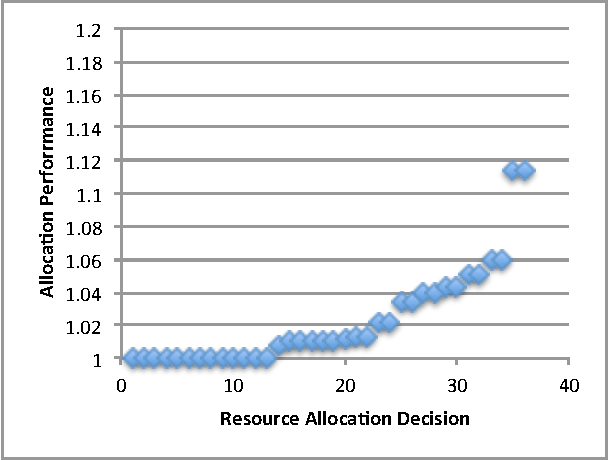
\includegraphics[width=.45\textwidth]{cluster_decision_points.pdf}
%		\caption{Performance of \pacora's NNLS algorithm}
%		\label{model_build_perf}
%	\end{center}
%\end{figure*}

To guarantee convexity of the RTF, the solution $w$ to $t \approx QRw$ must have no negative components.
Intuitively, when a resource is associated with more than a single $w_j$
or when the measured response time increases with allocation then negative $w_j$ may occur. \emph{Non-negative Least Squares} problems (NNLS) are common linear algebra, and there are several well-known techniques\cite{ChPl}.
However since \pacora's online model maintenance calls for
incremental downdates and updates to rows of $Q^T$, $Q^Tt$ and $R$,
the NNLS problem is handled with a scheme
based on the \emph{active-set} method\cite{LaHa} that
also downdates and updates the \emph{columns} of $R$ incrementally,
roughly in the spirit of Algorithm~3 in~\cite{LuDu}.
However, \pacora's algorithm cannot ignore downdated columns of $R$
because subsequent \emph{row} updates and downdates must have due effect
on these columns to allow their later reintroduction via column updates as necessary.
This problem is solved by leaving the downdated columns in place,
skipping over them in maintaining and using the QR factorization.

The memory used in maintaining a model with $n$ weights is modest, $24n^2 + 21n + \textrm{O}(1)$ bytes.
For $n = 8$ this is under 2 KB, fitting nicely in L1 cache.
Our NNLS implementation takes 4 $\micro$s per update-downdate pair in \tess.
%Figure~\ref{model_build_perf} shows the performance of \pacora's NNLS algorithm.

\subsubsection*{Model Rank Preservation}
If care is not taken in downdating $R$, its rows may become so linearly dependent,
perhaps from repetitive resource allocations,
that determining a unique $w$ is impossible.
The rank of $R$ depends on both the resource optimization trajectory and the
choices made in the row downdate-update algorithm.
\pacora exploits the latter idea and simply avoids downdating any row that will make $R$ rank-deficient.

\subsubsection*{Outliers and Phase Changes}

%\begin{figure*}[!t]
%	\begin{center}	
%%		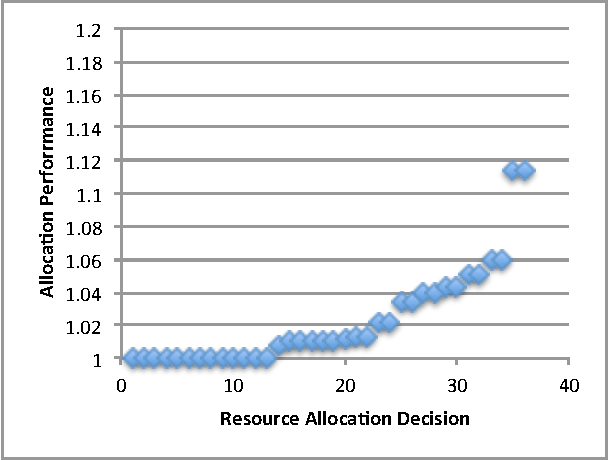
\includegraphics[width=.45\textwidth]{cluster_decision_points.pdf}
%		\caption{\pacora's online model creation algorithm adapting to a video application changing phases}
%		\label{phase_change}
%	\end{center}
%\end{figure*}

Some response time measurements may be ``noisy'' or even erroneous.
A weakness of least-squares modeling is the high importance it gives to outlying values.
On the other hand, when an application changes phase it is important to adapt quickly,
and what looks like an outlier when it first appears may be a harbinger of change.
What is needed is a way to discard either old or outlying data
with a judicious balance between age and anomaly.

The downdating algorithm accomplishes this by weighting the errors in $\varepsilon = Q(Q^Tt - Rw)$
between the predicted response times $\tau$ and the measured ones $t$ by a factor
that increases exponentially with the age $g(i)$ of the error $\varepsilon_i$.
Age can be modeled coarsely by the number of time quanta of some size since the measurement;
\pacora simply lets $g(i) = i$.
The weighting factor for the $i$th row is then $\eta^{g(i)}$ where $\eta$ is a constant somewhat greater than 1.
The candidate row to downdate is the row with the largest weighted error, \emph{i.e.,}
$dd = \arg\max_i |\varepsilon_i| \cdot \eta^{g(i)}$ and that does not reduce the rank of $R$.
%Figure~\ref{phase_change} shows \pacora's model creation algorithm adapting to a video application changing phases.


\subsubsection*{Power Response Modeling}
Recall that we manage power and battery energy with an artificial application named application 0 which receives all resources not allocated to other applications. Application 0's "response time" function is similar to the other applications' RTFs.  The function inputs are resource allocations just as with the other applications.  However, the function output is system power rather than response time.   To create the RTF, system power can be measured directly from on-chip energy counters in systems where they are available or from a power meter.  These models can be built in advance, during a training phase or online while the system runs, just as with the application RTFs.  Alternatively, the model could be part of the operating system's platform-specific information.

Although system power may not be perfectly convex in reality, forcing it to be convex is reasonable because idling a resource should not increase power.  As a result, application 0 still fufills its purpose of keeping applications from using additional resources that have poor performance/power ratios.


\section{Dynamic Penalty Optimization}\label{dyn_opt}

%IV.	Dynamic Optimization
%	a.	Gradient Descent w/ Backtracking Search
%		i. boundary conditions clean up
%	b.	Dealing with Fractional Results

\pacora's penalty optimization algorithm dynamically decides resource allocations. The algorithm can be run periodically, when applications start or stop, when an application changes faces or when the system changes operating scenarios.  One of the advantages of convex optimization is that it enables fast, incremental solutions.  As a result the algorithm could terminate earlier to decrease overhead and still be moving towards an optimal solution as it runs.  However we found in our implementation that the algorithm was fast enough to run to completion every time. 

Convex optimization is simplest when it is unconstrained, and so we reformulated \pacora's construction to be unconstrained.
Extending the response time model functions to all of $\Re^n$
moves the requirement that allocations must be positive into the objective function,
and introducing Application 0 for slack resources turns the affine inequalities into equalities:
\begin{eqnarray*}
& \makebox[1in][r]{Minimize}   & \sum_{p\epsilon P} {\pi_p(\tau_p(a_{p,1}\ldots a_{p,n}))}  \\
& \makebox[1in][r]{Subject to} & \sum_{p\epsilon P} a_{p,r} = A_r, r = 1,\ldots n           \\
\end{eqnarray*}

The only remaining constraints are those on the $a_{p,r}$.
These can be removed by letting the $a_{p,r}$ be unbounded above for $p \neq 0$
and changing the domain of $\tau_0$  to be the whole resource allocation matrix.
The definition of $\tau_0$ might take the form
\begin{eqnarray*}
\tau_0 &=& \sum_r \Delta_r \sum_{p \neq 0} a_{p,r}     \\
       &=& \sum_r \Delta_r (A_r - a_{0,r})
\end{eqnarray*}
where $\Delta_r$ is the (constant) power dissipation of one unit of resource $r$.
However,if any of the allocations $a_{0,r}$ turns out to be negative then $\tau_0$  should instead return the value $+\infty$.
This modification of the objective function transforms the resource allocation problem
to unconstrained convex optimization.  


The penalty optimization algorithm used in \pacora is gradient descent via backtracking line search along the negative gradient direction \cite{BoVa}.
This algorithm rejects and refines any step that yields insufficient relative improvement in the objective function,
so infinite values from infeasible allocations will automatically be avoided by the search.
The negative gradient $-\nabla\pi$ of the overall objective function $\pi$
with respect to the resource allocations $a$
is computed analytically from the response time models and penalty functions.
When a component of this overall gradient is negative,
it means the penalty will be reduced by increasing the associated allocation if possible.
The gradient search at the boundaries of the feasible region
must ignore components that lead in infeasible directions;
these can be detected by noting whether for some $p$ and $r$, $a_{p,r} = 0$ with $(-\nabla\pi)_{p,r} > 0$.
In such cases, the associated step component is set to zero.

We added an additional optimization to move along boundaries more rapidly in the scenario when a completely allocated resource had a large gradient.  We scale all the allocations of that resource type down to satisfy resource constraint while leaving the allocations of other resources untouched.

The rate of convergence of gradient descent depends on how well the sublevel sets of the objective function
are conditioned (basically, how ``spherical'' they are).
Conditioning will improve if resource allocation units are scaled to make their relative effects on $t$ similar.
For example, when compared with processor allocation units,
memory allocation units of 4MB are probably a better choice than 4 KB.
In addition, penalty function slopes should not differ by more than perhaps two orders of magnitude. If these measures prove insufficient, stronger preconditioners can be used. In our implementation, we condition all resource allocations to be in the range of 0-50.


\begin{figure*}[!t]
	\begin{center}	
%		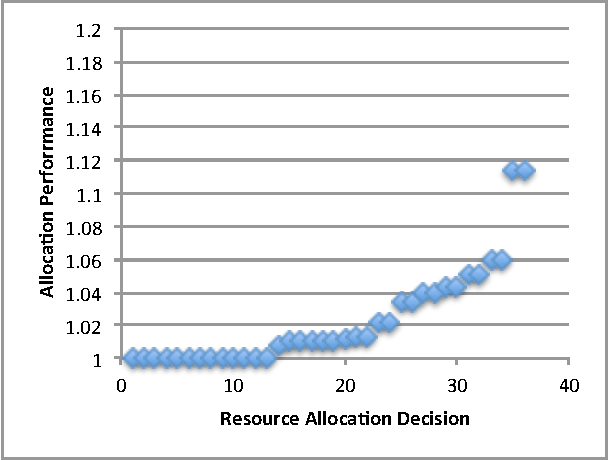
\includegraphics[width=.45\textwidth]{cluster_decision_points.pdf}
%		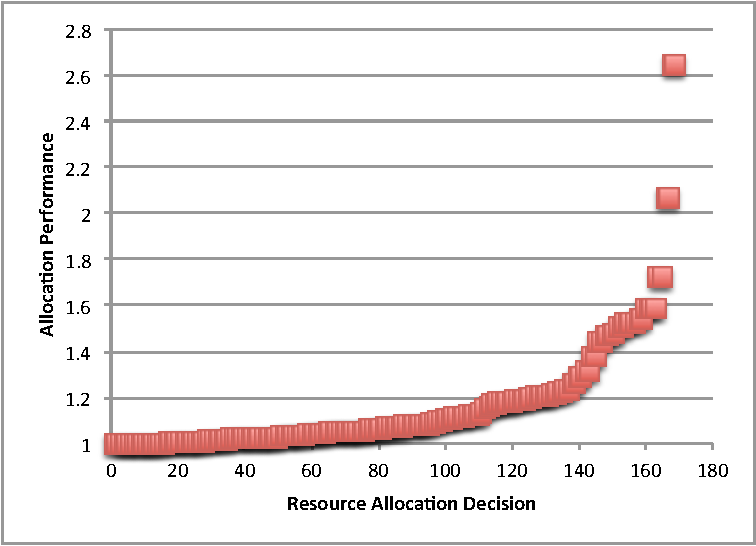
\includegraphics[width=.45\textwidth]{parsec_decision_points.pdf}
		\caption{Performance of our penalty optimization algorithm}
		\label{optimization_perf}
	\end{center}
\end{figure*}

Figure~\ref{optimization_perf} shows performance of penalty optimization algorithm implemented in \tess.  

%For our video conferencing scenario the average runtime is \fix{x} and then worst case runtime is \fix{y}.  \fix{explain where the variance comes from}

\section{Evaluation}

%V.	Evaluation
%	a.	Models
%		i.	Model Accuracy
%			1.	Matlab
%		ii.	Performance/Overhead
%			1.	Tess
%				a.	Time to build the model
%				b.	Phase Change Reaction
%		i.	Video Application adding threads
%		ii.	Time to react to phase changes
%		iii.	Show model accuracy through transition?
%	b.	Decisions
%		i.	Decision Accuracy
%			1.	Matlab
%		ii.	Performance/Overhead
%			1.	Tess
%	c.	Dynamic System
%		i.	Single Application � right sizing
%			1.	Without phase changes
%			2.	With phase changes
%			3.	Baseline � all allocations
%			4.	Measure Energy
%		ii.	Video, Animation, and Throughput Applications w/o phase changes
%			1.	Show throughput and missed deadlines for all the possible mixes
%			2.	Is it possible to show optimal?
%			3.	What is the baseline?
%		iii.	Video, Animation, and Throughput Applications w/ phase changes
%			1.	Show throughput and missed deadlines for all the possible mixes
%			2.	Basically just to show the system works


\cite{tess09}
\cite{SPEC2006}
\cite{parsec}
\cite{dacapo}
\cite{lithe}
\cite{matlab}
\cite{cvx}
%\cite{pulse}
\cite{bates-aes03}

PULSE (Preemptive User-Level SchEduling)
Lithe (LIquid THrEads)

\subsection{Experimental Methodology}
\label{sec:Platform}

To evaluate PACORA, we use two different implementations of the framework on the same hardware platform.  Our offline framework was used to experiment with the accuracy of different types of models and test

\subsubsection{Experimental Platform}

We use a prototype version of Intel's Sandy Bridge x86
processor to collect results on resource allocation and application
co-scheduling.  By using a real hardware prototype, we are able to run
full applications for realistic time scales and workload sizes, while running a standard operating system.  The processor is similar
to the commercially available client chip, but with additional
hardware to support way-based cache partitioning in the LLC.

The Sandy Bridge client chip has four quad-issue out-of-order
superscalar cores, each of which supports two hyperthreads using
simultaneous multithreading~\cite{IntelRefManual:2011}.  Each core has
private \wunits{32}{KB} instruction and data caches, as well as a
\wunits{256}{KB} private non-inclusive L2 cache.  The LLC is a 12-way
set-associative \wunits{6}{MB} inclusive L3 cache, shared among all
cores using a ring-based interconnect.  All three cache levels are
write-back.  Larger server versions of the same processor family have
up to \wunits{15}{MB} of LLC capacity.

The cache partitioning mechanism is way-based and modifies the
cache-replacement algorithm.  Each core can be assigned a subset of
the 12 ways in the LLC.  Although all cores can hit on data stored in
any way, a core can only replace data stored in one of its assigned
ways.  Allocation of ways among cores can be completely private,
completely shared, or overlapping.  Data is not flushed when the way
allocation changes; newly fetched data will just be written into one
of the assigned ways according to the updated allocation
configuration.

We use a customized BIOS that enables the cache partitioning
mechanism,

To measure on-chip energy, we use the energy counters available on
Sandy Bridge to collect the energy used by the entire socket and also
the total combined energy of cores, their private caches, and the
LLC. The counters measure power
at a $1/2^{16}$ second granularity.

\subsubsection{Offline Implementation}

and run unmodified Linux-2.6.36 for all of our experiments.
We use the Linux {\tt taskset} command to pin each application to
subsets of the available HyperThreads.

To measure application performance, we use the \texttt{libpfm}
library~\cite{Eranian:OLS06,Perfmon2}, built on top of the
\texttt{perf\_events} infrastructure introduced in Linux 2.6.31, to
access various performance-monitoring counters available on the
machine~\cite{Intel:Manual2012}.

We access these counters using the Running Average Power Limit
(RAPL) interfaces~\cite{Intel:Manual2012}.

\subsection{Description of Workloads}

We built our workload using a wide range of codes from three different
popular benchmark suites: SPEC CPU 2006~\cite{SPEC2006},
DaCapo~\cite{Blackburn:OOSPLA2006}, and PARSEC~\cite{Bienia:PdD2011}.
We included some additional application benchmarks to broaden the
scope of the study, and some microbenchmarks that exercise certain
features of the system.

The \textbf{SPEC CPU 2006} benchmark suite~\cite{SPEC2006} is a
CPU-intensive, single-threaded benchmark suite, designed to stress a
system's processor, memory subsystem and compiler.  Using the
similarity analysis performed by Phansalkar et
al.~\cite{Phansalkar:ISCA2007}, we subset the suite, selecting 4
integer benchmarks (astar, libquantum, mcf, omnetpp) and 4
floating-point benchmarks (cactusADM, calculix, lbm, povray).  Based
on the characterization study by Jaleel~\cite{Jaleel:TR2007}, we also
pick 4 extra floating-point benchmarks that stress the LLC: GemsFDTD,
leslie3d, soplex and sphinx3.  When multiple input sets and sizes are
available, we pick the single \textit{ref} input indicated by
Phansalkar et al.~\cite{Phansalkar:ISCA2007}. SPEC is the only
benchmark suite used in many previous characterizations of LLC
partitioning \cite{Suh:HPCA02,Qureshi:MICRO06,Guo:MICRO07}.

The \textbf{DaCapo} benchmark suite is intended as a tool for Java
benchmarking, consisting of a set of open-source, real-world
applications with non-trivial memory loads, including both client and
server-side applications. We used the latest 2009 release. The managed
nature of the DaCapo runtime environment has been shown to make a
significant difference in some scheduling studies \cite{Esmaeilzadeh:CACM2012}, and is
also representative of the increasing relevance of such runtimes.

The \textbf{PARSEC} benchmark suite is intended to be representative
of parallel real-world applications~\cite{Bienia:PdD2011}. PARSEC
programs use various parallelization approaches, including data- and
task-parallelization. We use the version of the benchmarks
parallelized with the {\tt pthreads} library, with the exception of
\texttt{freqmine}, which is only available in OpenMP. We used the full
native input sets for all the experiments. Past characterizations of
PARSEC have found it to be sensitive to available cache capacity
\cite{Bienia:PdD2011}, but also resilient to performance degradation in the face of
intra-application sharing of caches \cite{Zhang:PPoPP2010}.

We added four \textbf{additional parallel applications} to help ensure
we covered the space of interest: {\em Browser\_animation} is a
multithreaded kernel representing a browser layout animation; {\em
  G500\_csr} code is a kernel performing breadth-first search of a
large graph for the Graph500 contest, based on a new hybrid
algorithm~\cite{Beamer:EECS-2011}; {\em Paradecoder} is a parallel
speech-recognition application that takes audio waveforms of human
speech and infers the most likely word sequence intended by the
speaker; {\em Stencilprobe} simulates heat transfer through a fluid
using a parallel stencil kernel over a regular
grid~\cite{Kamil:Stencilprobe}.

\subsubsection{Manycore OS Implementation}













\subsection{Response-Time Functions}

\begin{figure*}[!t]
	\begin{center}	
%		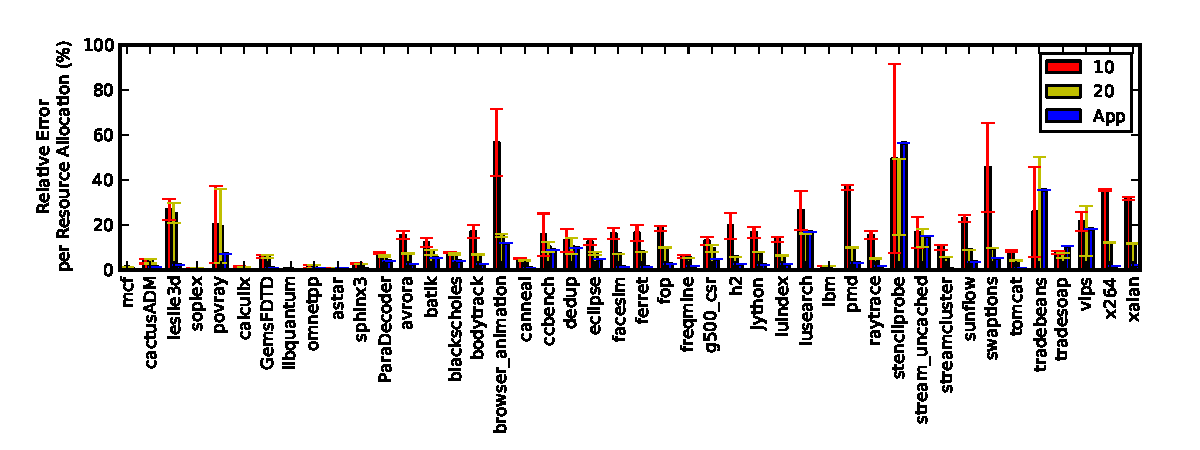
\includegraphics[width=\textwidth]{model_accuracy.pdf}
		\caption{L1 Norm of Relative Error of Response-Time model predicted runtime vs. actual runtime.  Data is from 3 complete trials.}
		\label{fig:model_accuracy}
	\end{center}
\end{figure*}
\begin{figure*}[!t]
	\begin{center}	
%		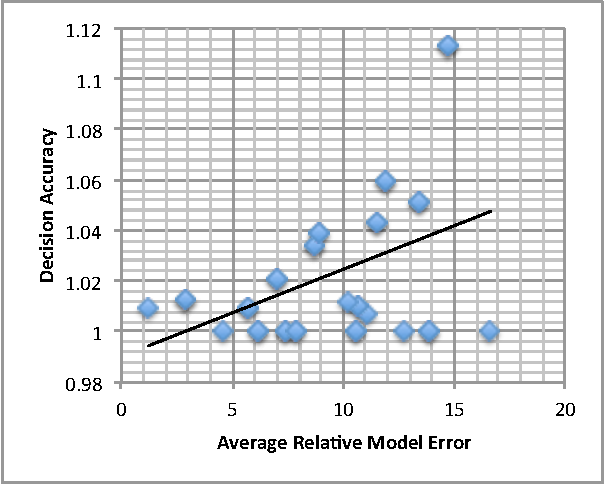
\includegraphics[width=.45\textwidth]{cluster_decision_accuracy.pdf}
%		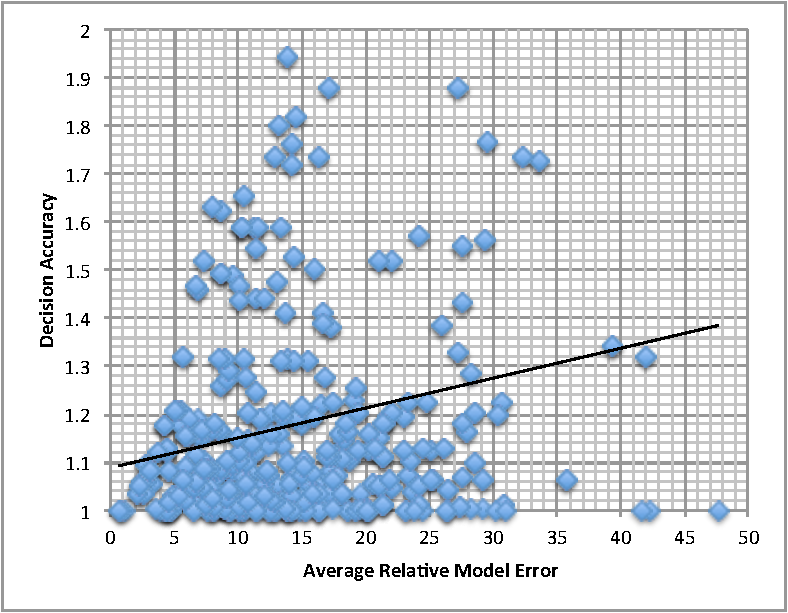
\includegraphics[width=.45\textwidth]{parsec_decision_accuracy.pdf}
		\caption{}
		\label{fig:model_accuracy}
	\end{center}
\end{figure*}


\subsection{Resource Allocation Decisions}
\begin{figure*}[!t]
	\begin{center}	
%		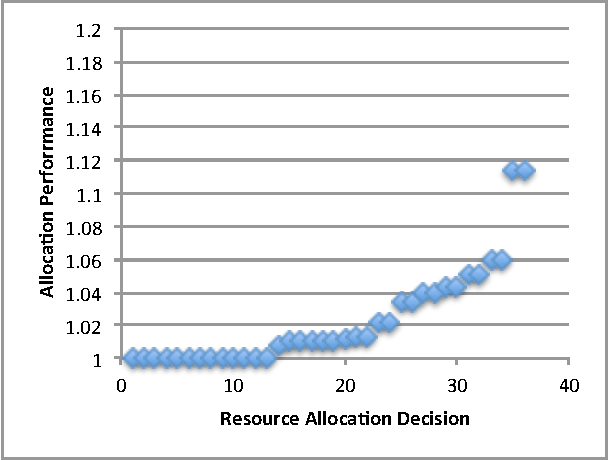
\includegraphics[width=.45\textwidth]{cluster_decision_points.pdf}
%		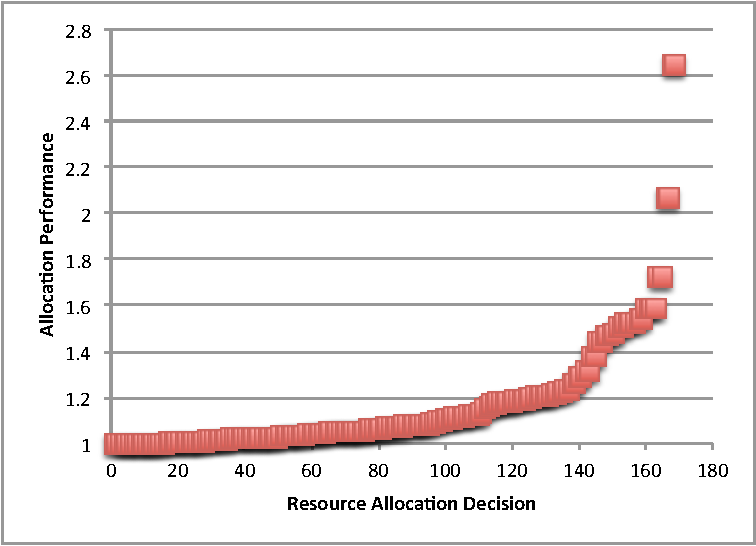
\includegraphics[width=.45\textwidth]{parsec_decision_points.pdf}
		\caption{}
		\label{fig:model_accuracy}
	\end{center}
\end{figure*}



%In addition, we use a FitPC external multimeter to measure the power
%consumed at the wall socket by the entire system, at a
%\wunits{1}{second} granularity.
%%Total system power is generally between \wunits{185}{W} and \wunits{240}{W}.
%The system-level values
%are correlated with data collected from the hardware energy counters
%using time stamps.  We observed less than one second of delay in these
%measurements consistently across all experiments.  Together, these
%mechanisms allow us to collect accurate energy readings over the
%entire course of an application's execution.

\section{Discussion}

\section{Related Work}\label{related_work}
\subsection{Batch Scheduling and Cluster Management}
Classic resource management systems were designed for batch scheduling~\cite{Feit97,FRS04}. Like \pacora, batch scheduling systems can allocate multiple resource types and rely on a gang-scheduling model~\cite{FeRu92}.  However, they tend to use queues and priorities to schedule jobs while trying to keep all resources busy. Resource allocations are always the user's responsibility to specify and pay for. Responsiveness can be improved by buying a higher priority. Few batch systems incorporate deadlines, but one such is \cite{AKKMS95}.

Modern cluster resource management has a similar flavor.  In systems such as
Amazon EC2~\cite{EC2}, Eucalyptus~\cite{eucalyptus}, and Condor~\cite{Condor}, users must specify their resource requirements.  Other systems such as Hadoop ~\cite{hadoop_fair, hadoop_cap, hadoop_matei} and Quincy~\cite{Quincy} use a fairness policy to assign resources. Mesos~\cite{mesos} uses two-level scheduling to manage resources in a cluster. Mesos decides how many resources to offer to its applications; they decide which resources to accept and how to schedule them. Mesos does not provide a particular resource allocation policy, but is a framework that can support multiple policies. Dominant Resource Fairness~\cite{mesos-DRF}, a generalization of max-min fairness to multiple resources types, has been implemented in Mesos.

\subsection{Model-Based Scheduling and Allocation Frameworks for SLAs and Soft Real-Time Requirements}

Research is growing in the cloud computing and realtime communities, which use application-specific performance ``models'' to try to schedule to meet deadlines or Service-Level Agreements (SLAs).

Much of this research has been in autonomic computing~\cite{1078472,1078493,1285843,1345325}. Typically, the performance models are utility functions derived from off-line measurements of raw resources utiilization. These functions are either interpolations from tables or analytic functions based on queueing theory.
%The utility functions typically map the number of servers each execution environment receives to its performance relative to its requirements, which may be several.
A central arbiter maximizes total utility. The utility functions are not necessarily concave,
so the arbiter must use reinforcement learning or combinatorial search to make allocations.
%Each application has a manager that schedules the resources given to it by the arbiter.
Walsh \emph{et al.}\cite{1078411} note the importance of basing utility functions
on the metrics in which QoS is expressed rather than on the raw quantities of resources.
There are other philosophical similarities to \pacora, but since the objective functions are discrete and non-convex their optimization is difficult. A survey of autonomic systems research appears in \cite{1380585}.

Rajkumar \emph{et al.}\cite{828990} propose a system Q-RAM that maximizes the weighted sum of utility functions, each of which is a function of the resource allocation to the associated application. Unlike \pacora, there is no distinction between performance and utility, and the utility functions are assumed as input rather than being discovered by the system. The functions are sometimes concave, and in these cases the optimal allocation is easily found by a form of gradient ascent. When the utility functions are not concave, a suboptimal greedy algorithm is proposed.
%They are always nondecreasing in every resource and sometimes are piecewise-linear and concave;

Several systems use a feedback-driven reactive approach to resource allocation where a control loop or reinforcement learning adjusts allocations continuously. AcOS\cite{AcOS} and Metronome\cite{Metronome} feature hardware-thread based maintenance of ``heart rate'' targets using adaptive reinforcement learning.
%AcOS also senses thermal conditions and can exploit Dynamic Voltage and Frequency Scaling (DVFS).
Bodik \emph{et al.}\cite{bodik-acdc09} builds on-line performance models like \pacora.
Initially, it uses an \emph{exploration policy} that avoids nearly all SLA violations while it builds the model; later, it shifts to a controller based on the model it has built.
The models are statistical, and bootstrapping is used to estimate performance variance.
Major changes in the application model are detected and cause model exploration to resume.
%The models are not convex or concave in general, and all SLAs must be met with high probability.

Jockey\cite{Jockey} has some similarities to \pacora: it is intended to handle parallel computation, its utility functions are concave,
and it adapts dynamically to application behavior.
Its performance models are obtained by calibrating either event-based simulation or a version of Amdahl's Law to computations.
Jockey does not optimize total utility but simply increases processors until utility flattens for each application,
\emph{i.e.,} each deadline is met.
A fairly sophisticated control loop prevents oscillatory behavior.

Other systems base decisions on user-provided resource specifications and a real-time scheduling algorithm.  In the Redline system\cite{Redline}, compact resource requirement specifications written by hand to guarantee response times are scheduled Earliest-Deadline-First.
%Isolation of resources is strong, as in \pacora.  Scheduling is Earliest-Deadline-First.
%Admission control is lenient but oversubscription situations are remedied by de-admitting some of the non-interactive applications.

Much research focuses on measuring resource usage to make smart co-scheduling decisions.
For example, Calandrino \emph{et al.}\cite{unc} uses working set sizes to make co-scheduling decisions and enhance soft real-time behavior. Merkel and Bellosa\cite{merkel-eurosys08} propose \emph{Task Activity Vectors} that describe how much each application uses the various functional units; these vectors are used to balance usage across multiple cores.
%and unbalance usage among hardware threads within each core.
%The intended effect is to distribute chip temperature more evenly, but the idea may be more broadly applicable, \emph{e.g.,} for heterogeneous systems.

 Some frameworks can support multiple scheduling and resource allocation policies. Guo \emph{et al.}\cite{1331730} present such a framework.  They point out that much prior work is insufficient for true QoS; merely partitioning hardware is not enough because there must also be a way to specify performance targets and an admission control policy for jobs. Unlike \pacora, they argue that targets should be expressed in terms of capacity requirements rather than rates or times.

Nesbit \emph{et al.}\cite{1436097} introduces \emph{Virtual Private Machines} (VPM), a framework for resource allocation and management in multicore systems. A VPM comprises a set of virtual hardware resources, both spatial (physical allocations) and temporal (scheduled time-slices).
%They break down the framework components into policies and mechanisms which may be implemented in hardware or software.
VPM \emph{modeling} maps high-level application objectives via \emph{translation}, which uses models to assign acceptable VPMs to applications while adhering to system-level policies. A \emph{scheduler} decides if the system can accommodate all applications. The VPM approach and terminology are similar to \pacora's at a high level.  However, Nesbit \emph{et al.} did not perform design, implementation or evaluations of the modeling, translation, or scheduling components suggested in their paper.

%mesh well with our study, which can be seen as a specific implementation of several key aspects of the type of framework they describe (i.e. VPM modeling and translation).
%
%Unlike traditional virtual machines that only virtualize resource functionality, VPMs virtualize a system's performance and power characteristics, meaning that a VPM has the same performance and power profile as a real machine with an equivalent set of hardware resources.

\subsection{Resource Partitioning and QoS}
\label{sec:rel:pm}

\pacora relies on resource partitioning and Quality-of-Service mechanisms when available to enforce its resource allocation decisions.  Resource partitioning and QoS research is active for on-chip, cluster, and networking resources.  However, the vast majority of research focuses on allocating a single resource type with a fixed policy, typically \emph{fairness}.
Some have researched network bandwidth fairness~\cite{Blanquer, Kleinberg99fairnessin, Liu}, while others~\cite{Baruah96proportionateprogress, Baruah_fastscheduling, Zhu} have concentrated on CPU fairness.

Hardware partitioning research, which has largely focused on caches, provides mechanisms based on policies baked into the hardware, not the flexible allocations \pacora requires \cite{876484, 967444,1194855,1275005,1194858,1318096,1088154,1399973,1069998,1399982}.  Early work focused on providing adaptive, fair policies that ensure equal performance degradation \cite{605420,1086328}, not guarantees of responsiveness. More recent proposals have incorporated more sophisticated policy management \cite{1241608,1331730,1152161,1254886}. Iyer\cite{1006246} suggests a priority-based cache QoS framework, CQoS, for shared cache way-partitioning.
%The priorities might be specified per core, per application, per memory type, or even per memory reference.
However, simultaneous achievement of performance targets as in \pacora is not addressed.


%In general, these papers focus on designing and proving the effectiveness of particular mechanisms for particular goalswithout a concrete notion of a general-purpose resource allocation or scheduling framework.
%in which a variety of application-specific QoS requirements can be communicated to an all-purpose resource allocator and scheduler.



%The Singularity operating system\cite{aiken-mspc06} provides process isolation through software rather than hardware.  This isolation in accessibility is not the same as the performance isolation that is desirable for \pacora.

%Other partitioning work has focused on interconnect bandwidth QoS \cite{1382130} or partitioning cache capacity and bandwidth simultaneously \cite{1250671}.

%CQoS: a framework for enabling QoS in shared caches of CMP platforms
%\cite{1006246}

%Suh \emph{et al.}\cite{876484, 967444} and Qureshi and Patt \cite{1194855} monitor individual applications' cache performance to decide partitioning in an attempt to reduce the total amount of cache misses and off-chip memory traffic.
%A wide variety of proposals exist for multicore last-level cache structures that partition the spatial resources between private and shared data, in an attempt to create a manageable trade-off between capacity for shared data and low latency for private data \cite{1275005,1194858,1318096,1088154,1399973,1069998,1399982}.

%\subsection{Application Performance Modeling}
%
%\fix{add information here}


%Citations supporting PACORA's assumptions.

%Ganapathi \emph{et al.} have had success using machine learning to model application performance and select the best performing configuration in \cite{Archana}.

%Kumar \emph{et al.}\cite{1006707} demonstrate the performance advantages of heterogeneous cores for mixed workloads using heuristic allocation strategies in both space and time.
%
%Genbrugge and Eeckhout\cite{genbrugge-isca07} demonstrate the importance of adapting to changes in application characteristics, in this case instructions per cycle.

%\todo{I DON'T KNOW WHY \cite{975344,wasserman-book} ARE IN HERE}

%Scheduling threads for constructive cache sharing on CMPs
%\cite{1248396}
%
%Chen \emph{et al.}\cite{1248396} propose parallel depth-first thread scheduling as an alternative to work-stealing for constructive cache sharing.
%The paper discusses the automation of task granularity selection to match cache capacity. This kind of tuning is particularly appropriate for a user-level runtime system.


%\subsection{Autonomic Systems}
%Resource Allocation for Autonomic Data Centers using Analytic Performance Models
%	\cite{1078472}
%	
%Autonomic QoS-aware resource management in grid computing using online performance models
%	\cite{1345325}
%
%On the use of hybrid reinforcement learning for autonomic resource allocation
%\cite{1285843}
%	
%Utility-Function-Driven Resource Allocation in Autonomic Systems
%\cite{1078493}

%Redline: First Class Support for Interactivity in Commodity OSs \cite{Redline}
%Paper presented in OSDI'08.
%

%Jockey: Guaranteed Job Latency in Data Parallel Clusters \cite{Jockey}
%Work from Microsoft about the system they built on top of their Cosomos cluster (Dryad???)

%Discusses how they do the dynamic resource allocation for jobs running in a cluster
%Paper from Eurosys 2012
%


%Automatic Exploration of Datacenter Performance Regimes
%\cite{bodik-acdc09}
%

%AcOS: an Autonomic Management Layer Enhancing Commodity Operating Systems \cite{AcOS}
%Work at the Politecnico di Milano, Italy.
%Master Thesis
%Paper and slides at the CHANGE 2012 Workshop (DAC)
%
%Metronome: OS Level Performance Management via Self Adaptive Computing \cite{Metronome}
%Work related to AcOS, done by people from the Politecnico di Milano (Italy), MIT and Harvard.
%Paper presented in DAC 2012.

%A resource allocation model for QoS management
%\cite{828990}
%

%Utility-Based Cache Partitioning: A Low-Overhead, High-Performance, Runtime Mechanism to Partition Shared Caches
%\cite{1194855}
%


\section{Conclusion}


\bstctlcite{bstctl:etal, bstctl:nodash, bstctl:simpurl}
\bibliographystyle{IEEEtranS}
\bibliography{references}

\end{document}

